%!TEX root = course-work6-paper.tex
% Добавьте ссылку на файлы с текстом работы
% Можно использовать команды:
%   \input или \include
% Пример:
%    \input{mainfiles/1-section} или \include{mainfiles/2-section}
% Команда \input позволяет включить текст файла без дополнительной обработки
% Команда \include при включении файла добавляет до него и после него команду
% перехода на новую страницу. Кроме того, она позволяет компилировать каждый файл
% в отдельности, что ускоряет сборку проекта.
% ВАЖНО: команда \include не поддерживает включение файлов, в которых уже содержится команда \include,
% т.е. не возможен рекурсивный вызов \include
\newcommand*{\Source}{
    % \subsection*{\centeringАннотация}
В данной работе рассматриваются современные подходы по распознаванию семантики кода. 

TODO
\newpage

    \section*{Введение} 
\addcontentsline{toc}{section}{Введение}
Потребность в анализе исполняемого кода возникает у любого специалиста, пытающегося провести анализ достаточно большой программы в отсутствие исходного кода с целью достичь понимания ее устройства. Подобная ситуация возникает при изучении вредоносного кода разработчиками антивирусов, при оценке свойств алгоритмов во время сертификационных испытаний, восстановлении закрытых протоколов для их последующей реализации в программах с открытым исходным кодом, выявлении ошибок и выделении среди них уязвимостей и т.п.

Упомянутая выше задача анализа исполняемого кода является частным случаем более общей задачи исследования семантики кода. Полученный результат может быть использован для решения многих практических задач:
\begin{itemize}
	\item Автоматическая проверка кода -- рекомендация названий имен функций может улучшить читаемость и поддержку кода и упростить использование открытого API, также может использоваться для подсказки правильного названия метода при разработке в IDE;
	\item Автодополнения кода;
	\item Генерация кода;
	\item Распознавание дублирования кода;
	\item Предсказание оптимальных параметров для запуска программы;
	\item Определение класса алгоритма (ускорение reverse-engineering) и др.
\end{itemize}

В последние годы методы машинного обучения стали применяться для большего спектра задач, в частности для задачи анализа исходного и исполняемого кода. Среди прочего, используются методы на основе нейросетей, которые имеют ряд преимуществ. Так, например, нейросеть может тренироваться для решения конкретной задачи, для которой ей могут потребоваться лишь определенные признаки исходного набора данных (это полезно, если набор данных собирается вручную, и генерация некоторых признаков может быть сильно затратной). Следующим достоинством является то, что одна и та же нейросеть может быть обучена на разных наборах данных и может решать несколько разных задач. Вычисление результата предсказания может быть произведено быстро из-за эффективной параллельной реализации на графическом ускорителе. Однако у этих методов есть некоторые недостатки. Одним из условий для применения нейросетей является необходимость наличия большого размеченного набора данных.

Для задач, связанных с исходным кодом, существует множество различных размеченных наборов данных, следовательно указанное ограничение не является проблемой. Однако для задач, связанных с бинарным кодом, проблема стоит достаточно остро. Во-первых, работ по данной тематике не очень много, а наборов данных на популярном ресурсе \footnote{\url{https://paperswithcode.com/}}, содержащем ссылки на статьи с кодом, и вовсе нет. Кроме того, не были найдены наборы данных на сервисе \footnote{\url{https://datasetsearch.research.google.com/}}. Во-вторых, в одних работах авторы используют лишь некоторую статистику, собранную по исполняемым файлам (например, частоты встречаемости байтов или инструкций), а в других - решают задачу на ''модельных'', т.е либо небольших, либо нерепрезентативных, наборах данных. Поиск большого размеченного набора данных из реальных проектов не дал результатов.

В дипломной работе был предложен метод классификации функций в бинарных файлах, который был опробован на декомпилированном наборе данных POJ-104\cite{DBLP:journals/corr/MouLJZW14}. Однако сам набор данных был модельным. Во-первых, в нем были классы, в которых основой частью алгоритма являлась сортировка по ключу, а сами классы отличались лишь структурами. Во-вторых, некоторые классы содержали очень специфичные или мало отличающиеся друг от друга программы. Например, были представлены следующие классы программ: класс программ реализующих удаление подряд идущих пробелов, и класс программ, ищущих все простые числа на заданном отрезке.

В настоящей работе для проверки работоспособности метода на реальных данных было принято решение о самостоятельной сборке набора данных, удовлетворяющего описанным выше требованиям.
    \section{Цель работы}
Целью данной работы является сбор размеченного для классификации набора данных из бинарного кода функций и проверка применимости предложенного для классификации метода. 

\subsection{Постановка задачи}
Для достижения заданной цели были поставлены следующие задачи:
\begin{enumerate}
	\item Исследовать современные подходы, основанные на машинном обучении, применительно к задаче понимания семантики кода;
	\item Собрать набор данных, состоящий из бинарного кода функций из промышленных проектов;
	\item Определить множество классов, отражающих семантику собранных функций;
	\item Произвести разметку собранных данных по полученному множеству классов;
	\item Протестировать метод для классификации на полученном наборе данных.
\end{enumerate}
    \section{План решения задачи}
Для решения поставленных задач был составлен следующий план (подробное объяснение плана представлено в секции \ref{5-dataset}).
\begin{enumerate}
    \item Рассмотреть современные подходы для классификации исходного кода и возможность их применения для классификации бинарного кода;
    \item Написать краулер для сбора проектов на языке Rust с платформы Github;
    \item Выбрать сигнатуры функций и комментарии к ним из собранного кода;
    \item \label{class_selection} Выделить классы в предположении, что в реальных проектах полученные данные достаточно хорошо могут описывать семантику функций;
    \item Для полученного размеченного набора данных применить метод классификации, предложенный ранее.
\end{enumerate}

Остановимся подробнее на п.\ref{class_selection} плана.

\subsection{Выделение классов}
Сначала произвести предобработку данных:
\begin{enumerate}
    \item Имена функций, семантически состоящие из нескольких слов, разбить на части перебором по различным стилям написания (camelCase, underscores, PascalCase);
    \item Привести слова к нижнему регистру, удалить все символы-цифры;
    \item Произвести сегментацию полученных слов, так чтобы вероятность полученного разбиения была максимальной;
    \item Произвести лемматизацию;
    \item Удалить слишком короткие, длинные, редкие и частые слова.
\end{enumerate}

Далее полученные токенизированные представления функций перевести в векторы с помощью tf-idf. Затем применить методы для тематической классификации (LSA, PLSA, LDA...) либо использовать алгоритмы кластеризации (k-means, DBSCAN и др.). После этого вручную отобрать полученные классы.
    \section{Описание предметной области}
В дальнейшем тексте будут неоднократно использоваться различные понятия из машинного обучения и внутреннего представления LLVM IR. В этой секции приводится краткое описание предметной области.

\subsection{Связь с обработкой естественных языков}
Рассмотрим сначала, как именно машинное обучение может быть применимо к задаче анализа исходного кода. В области машинного обучения и искусственного интеллекта есть направление ответвление, занимающееся обработкой естественного языка (Natural Language Processing, NLP), которое изучает проблемы компьютерного анализа и синтеза естественных языков. Код на языке программирования является искусственным языком, имеющим строгий синтаксис и семантику, в отличие от естественного языка. Искусственный и естественный языки имеют и другие отличия, однако существует гипотеза, что тексты на языке программирования имеют некоторые статистические особенности, схожие с текстами на естественном языке, и эти особенности могут быть использованы для построения инструментов анализа кода программ. Поэтому существуют методы обработки текстов, которые могут также быть применены к анализу исходного кода программ. 

\subsection{Векторное представление слов}
Во многих методах обработки текстов на естественном языке с помощью машинного обучения используется подход, направленный на получение представления единицы текста (слова, предложения и т.п.) в виде вещественного вектора. Это так называемое векторное представление слов (embedding). Основной целью данного подхода является получение признаков, представляющих информацию об исходных текстах в пригодном для метода формате, т.к. большинство методов машинного обучения принимают на вход в качестве признаков набор вещественных векторов.

\subsection{LLVM}
LLVM\cite{Lattner:MSThesis02} -- проект программной инфраструктуры для создания компиляторов и сопутствующих им утилит. Состоит из набора компиляторов из языков высокого уровня, системы оптимизации, интерпретации и компиляции в машинный код. В основе инфраструктуры используется RISC-подобная платформонезависимая система кодирования машинных инструкций -- байткод LLVM IR, которая представляет собой высокоуровневый ассемблер, с которым работают различные преобразования. Над промежуточным представлением можно производить трансформации во время компиляции, компоновки и выполнения. Из этого представления генерируется оптимизированный машинный код для целого ряда платформ как статически, так и динамически.

Проект LLVM написан на C++ и портирован на большинство Unix-подобных систем и Windows. Система имеет модульную структуру, отдельные её модули могут быть встроены в различные программные комплексы, она может расширяться дополнительными алгоритмами трансформации и кодогенераторами для новых аппаратных платформ.

\subsection{LLVM IR}
LLVM IR -- это промежуточное представление в виде трёхадресного кода в SSA-форме. На практике для хранения кода используется эффективное бинарное представление (bitcode). SSA -- это такая форма промежуточного представления кода, в которой любое значение присваивается только один раз.

LLVM IR поддерживает следующие типы данных:
\begin{itemize}
    \item Целые числа произвольной разрядности. Генерация машинного кода для типов очень большой разрядности не поддерживается, но для промежуточного представления никаких ограничений нет;
    \item Числа с плавающей точкой: float, double, а также ряд типов, специфичных для конкретной платформы (например, x86$\_$fp80);
    \item void -- пустое значение;
    \item Указатели;
    \item Массивы;
    \item Структуры;
    \item Функции;
    \item Векторы.
\end{itemize}

Система типов рекурсивна, поэтому можно использовать многомерные массивы, массивы структур, указатели на структуры и функции, и т.д.

Большинство инструкций в LLVM принимают два аргумента и возвращают одно значение. Значения определяются текстовым идентификатором. Локальные значения обозначаются префиксом $\%$, а глобальные -- @. Локальные значения также называют регистрами, а LLVM -- виртуальной машиной с бесконечным числом регистров.

Тип операндов всегда указывается явно, и однозначно определяет тип результата. Операнды арифметических инструкций должны иметь одинаковый тип, но сами инструкции «перегружены» для любых числовых типов и векторов.
Всего существует 52 инструкции, среди них:
\begin{itemize}
    \item набор арифметических операций;
    \item набор побитовых логических операций и операций сдвига;
    \item специальные инструкции для работы с векторами;
    \item инструкции для обращения к памяти;
    \item операции приведения типа.
\end{itemize}

Из этого краткого обзора видно, что промежуточное представление LLVM достаточно близко соответствует коду на низкоуровневых процедурных языках наподобие Си. При трансляции высокоуровневых языков -- объектно-ориентированных, функциональных, динамических -- придётся выполнить гораздо больше промежуточных преобразований, а также написать специализированный интерпретатор. Но и в этом случае LLVM снимает с разработчика компилятора проблемы кодогенерации для конкретной платформы, берёт на себя большинство независимых от языка оптимизаций и делает их качественно. Кроме этого, с помощью LLVM разработчик получает готовую инфраструктуру для динамической компиляции и возможность оптимизации времени связывания между различными языками, компилируемыми в LLVM.

\subsection{Ida}
IDA Pro Disassembler -- интерактивный дизассемблер, который широко используется для реверс-инжиниринга. Он отличается исключительной гибкостью, наличием встроенного командного языка, поддерживает множество форматов исполняемых файлов для большого числа процессоров и операционных систем. Позволяет строить блок-схемы, изменять названия меток, просматривать локальные процедуры в стеке и многое другое.

IDA до определенной степени может автоматически выполнять анализ кода, используя перекрестные ссылки (xref's), знание параметров вызовов функций стандартных библиотек и другую информацию. Однако одной из самых главных его особенностей считается удобное интерактивное взаимодействие с пользователем. В начале исследования IDA выполняет автоматический анализ программы, а затем пользователь с помощью интерактивных средств начинает давать осмысленные имена, комментировать, создавать сложные структуры данных и другим образом добавлять информацию в листинг, генерируемый дизассемблером, пока не станет ясно, что именно и как делает исследуемая программа.

Дизассемблер имеет консольную и графическую версии. Поддерживает большое количество форматов исполняемых файлов. Одной из отличительных особенностей IDA Pro является возможность дизассемблирования байт-кода виртуальных машин Java и .NET. Также поддерживает макросы, плагины и скрипты, а последние версии содержат интегрированный отладчик.\cite{Ida}

Ida Pro является одним из самых популярных дизассемблеров по нескольким причинам:
\begin{enumerate}
    \item Для Ida существует множество плагинов на языках IDC и Python, например восстановление AST-дерева программы;
    \item Ida использует огромное число эвристик и техник, использующихся при компиляции;
    \item Ida сама комментирует код и распознает стандартные библиотечные и системные функции;
    \item Интерактивность процесса дизассемблирования.
\end{enumerate}

\subsection{Mcsema}
Mcsema\cite{Mcsema} -- это фреймворк, который позволяет переводить бинарный исполняемый файл в llvm биткод.

McSema дает аналитику возможность найти в программе уязвимости, которые очень сложно отследить в исполняемом файле, независимо проверить исходный код поставщика программы и составить тесты с большим покрытием кода. Также оттранслированный LLVM биткод может быть подвержен тестированию с помощью libFuzzer\cite{libFuzzer}. Кроме того, полученный биткод можно скомпилировать в исполняемый бинарный файл.

McSema поддерживает трансляцию ELF и PE форматов исполняемых файлов, а также большинство x86 и amd64 инструкций, включая X87, MMX, SSE и AVX.

Процесс получения llvm биткода состоит из двух шагов: восстановления графа потока управления и трансляции инструкций. Восстановление графа потока управления осуществляется с использованием программы mcsema-disass, которая использует один из следующих дизассемблеров: IDA Pro, Binary Ninja или DynInst. Трансляция инструкций выполняется с помощью программы mcsema-lift, которая переводит граф потока управления в LLVM биткод.

    \section{Обзор литературы}
Задача автоматизированного выявления паттернов в бинарных программах известна достаточно давно (одной из первых работ в этой области является \cite{bugs}). Существующие способы решения используют в основном статический и динамический анализ, основанный на различных эвристиках. Но сравнительно недавно стали очень активно развиваться методы анализа, основанные на машинном обучении. В этом разделе рассматриваются несколько существующих на данный момент подходов по распознаванию семантики исходного кода с анализом их плюсов и минусов в контексте применения для выявления паттернов в скомпилированных бинарных программах.

\subsection{Graph2Seq}
В данной статье\cite{xu2018graph2seq} авторы представляют модель типа кодер-декодер для перевода входных данных в виде графа в последовательность. Сначала к графу применяются сверточные слои с нелинейными активациями, затем с помощью операции пуллинга всех векторных представлений получается векторное представление графа. Полученное векторное представление передается на вход рекуррентной нейронной сети с механизмом внимания. Авторы получили лучшие или близкие к лучшим результаты для 3 задач: первые две относились к поиску кратчайшего пути в графе, последняя к переводу запросов языка SQL в описание на естественном языке. Ниже представлена схема, описывающая работу данной модели:
\begin{figure}[h]
    \center{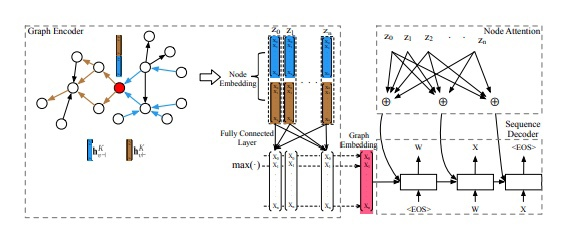
\includegraphics[width=0.9\linewidth]{images/GRAPH2SEQ.jpg}}
    \caption{Схема модели graph2seq}
\end{figure}

Эта модель может быть с небольшими изменениями адаптирована для задачи graph2vec, например, если совсем убрать декодер, или полученную последовательность подать на вход модели seq2vec. При этом во втором случае элементы последовательности будут содержать информацию о всем графе, и каждый элемент последовательности сильнее учитывает значение соответствующей вершины в исходном графе.

\subsection{Improved Code Summarization via a Graph Neural Network}
В работе\cite{leclair2020improved} авторы решали задачу суммаризации кода, основываясь на работе graph2seq. Модель представляет собой кодер-декодер с несколькими входами. Модель последовательно предсказывает текст-описание функции, на каждой итерации получает на вход последовательность токенов кода, его абстрактное синтаксическое дерево и предсказанную до текущего момента последовательность. Затем токены переводятся в соответствующие векторные представления и подаются на вход GRU. Абстрактное синтаксическое дерево с соответствующими векторными представлениями проходят 2 сверточных слоя и подаются на вход GRU. Предсказанная к текущему моменту последовательность переводится в векторные представления и подается на вход GRU. Далее полученные последовательности соответствующие абстрактному синтаксическому дереву и предсказанной последовательности передаются в механизм внимания. Аналогично обстоит дело с последовательностью, соответствующей исходным токенам. Затем полученные векторы объединятся, подаются в линейный слой. Полученный вектор можно использовать для предсказания следующего токена.
\begin{figure}[h]
    \center{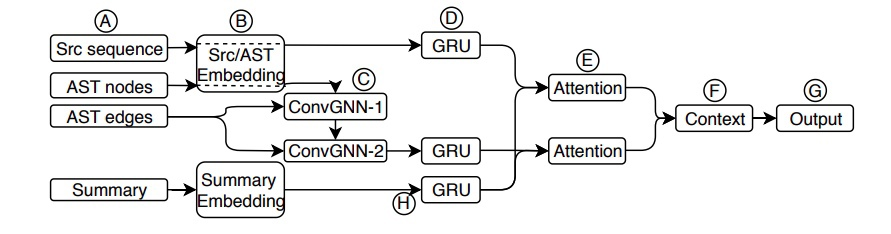
\includegraphics[width=0.9\linewidth]{images/gnn1.jpg}}
    \caption{Модель использующая GCN для суммаризации}
\end{figure}

\subsection{Retrieval-Augmented Generation for Code Summarization via Hybrid GNN}
В работе\cite{liu2021retrievalaugmented} авторы также решали задачу суммаризации кода. Модель представляет собой кодер-декодер. Модель работает следующим образом:
\begin{itemize}
    \item По имеющемуся исходному коду строится CPG граф\cite{6956589}, последовательность признаков вершины и ее тип кодируются с помощью матриц векторных представлений. Преобразованная последовательность признаков подается в двунаправленный LSTM блок;
    \item
        \begin{itemize}
            \item Ищется наиболее похожий код в имеющемся обучающем наборе данных;
            \item Вычисляется матрица внимания на основе всех векторных представлений вершин найденного кода и исходного; Полученная матрица умножается на коэффициент схожести найденного кода и матрицу векторных представлений найденного кода. Эта матрица прибавляется к матрице исходного кода;
            \item Описание для найденного кода кодируется с помощью векторных представлений и подается в двунаправленный LSTM блок. Позже выход LSTM умножается на коэффициент близости, конкатенируется с выходом GNN и подается в декодер.
        \end{itemize}
    \item Строится динамический граф (точнее, его матрица смежности) на основе механизма внимания, чтобы была возможность передачи информации между двумя произвольными вершинами. Затем нормализуется;
    \item Вычисляются векторы агрегированные векторы после свертки на статическом и динамическом графах, вычисляется взвешенная сумма с вычисляемыми коэффициентами и подается на вход GRU блоку;
    \item Декодер представляет из себя LSTM и получает на вход векторы из GRU и поданного в LSTM блок описания для ближайшего найденного кода.
\end{itemize}

\begin{figure}[h]
    \center{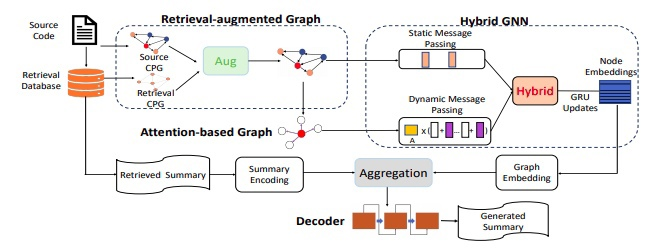
\includegraphics[width=0.8\linewidth]{images/HGNN.jpg}}
    \caption{Hybrid GNN}
\end{figure}

\subsection{Inst2vec}
Используя метод inst2vec\cite{ncc} авторы предложили решение сразу 3 задач. Первая задача состояла в определении класса алгоритма. Во второй задаче надо было определить, на каком вычислительном устройстве (центральный процессор или видеокарта) выгоднее запустить программу, чтобы ее время исполнения было меньше. Третья задача заключалась в определении максимального количества нитей при запуске кода на видеокарте для минимизации времени работы. Для решения этих задач использовался подход с обучением векторного представления инструкций.

Т.к. исходный код для этих задач может быть написан на разных высокоуровневых языках, то с целью генерализации подхода авторы выбрали представление llvm ir, в которое может быть скомпилирован код на большом множестве языков, например, на C/C++, FORTRAN, Python, Java, CUDA, OpenCL и др. Было сделано предположение, что инструкции, которые находятся "близко" друг к другу, имеют похожий смысл. Поэтому для обучения векторных представлений были выбраны модели Word2vec\cite{DBLP:journals/corr/MikolovSCCD13} и Skip-Gram, использование которых предполагает наличие понятия контекста слова(в данном случае инструкции).

Авторы определяют контекст инструкции, как множество инструкций, от которых напрямую зависит выполнение данной инструкции. Таким образом учитывается зависимость как по передаче управления, так и зависимость по данным. Инструкции с вышеупомянутой зависимостью не могут быть напрямую извлечены из исходного кода, поэтому сначала строится XFG (contextual-flow graph) граф. Это ориентированный мультиграф, который определяется следующим образом: вершинами являются переменные или метки, например, базовые блоки, функции; ребра являются либо зависимостью по данным либо зависимостью по управлению; если у инструкции нет зависимости по данным, она соединяется ребром с корневой вершиной. Для того, чтобы словарь не был очень большим данные подвергались предобработке. Убирались комментарии и метаданные, константы заменялись на фиксированные токены, имена переменных заменялись на специальный токен, производилась подстановка структур.

После обучения векторных представлений для решения поставленных задач обучалась рекуррентная нейронная сеть, которая принимала на вход преобразованную в векторное представление последовательность инструкций llvm ir (рисунок \ref{ris:inst2vec}).
\begin{figure}[h]
    \center{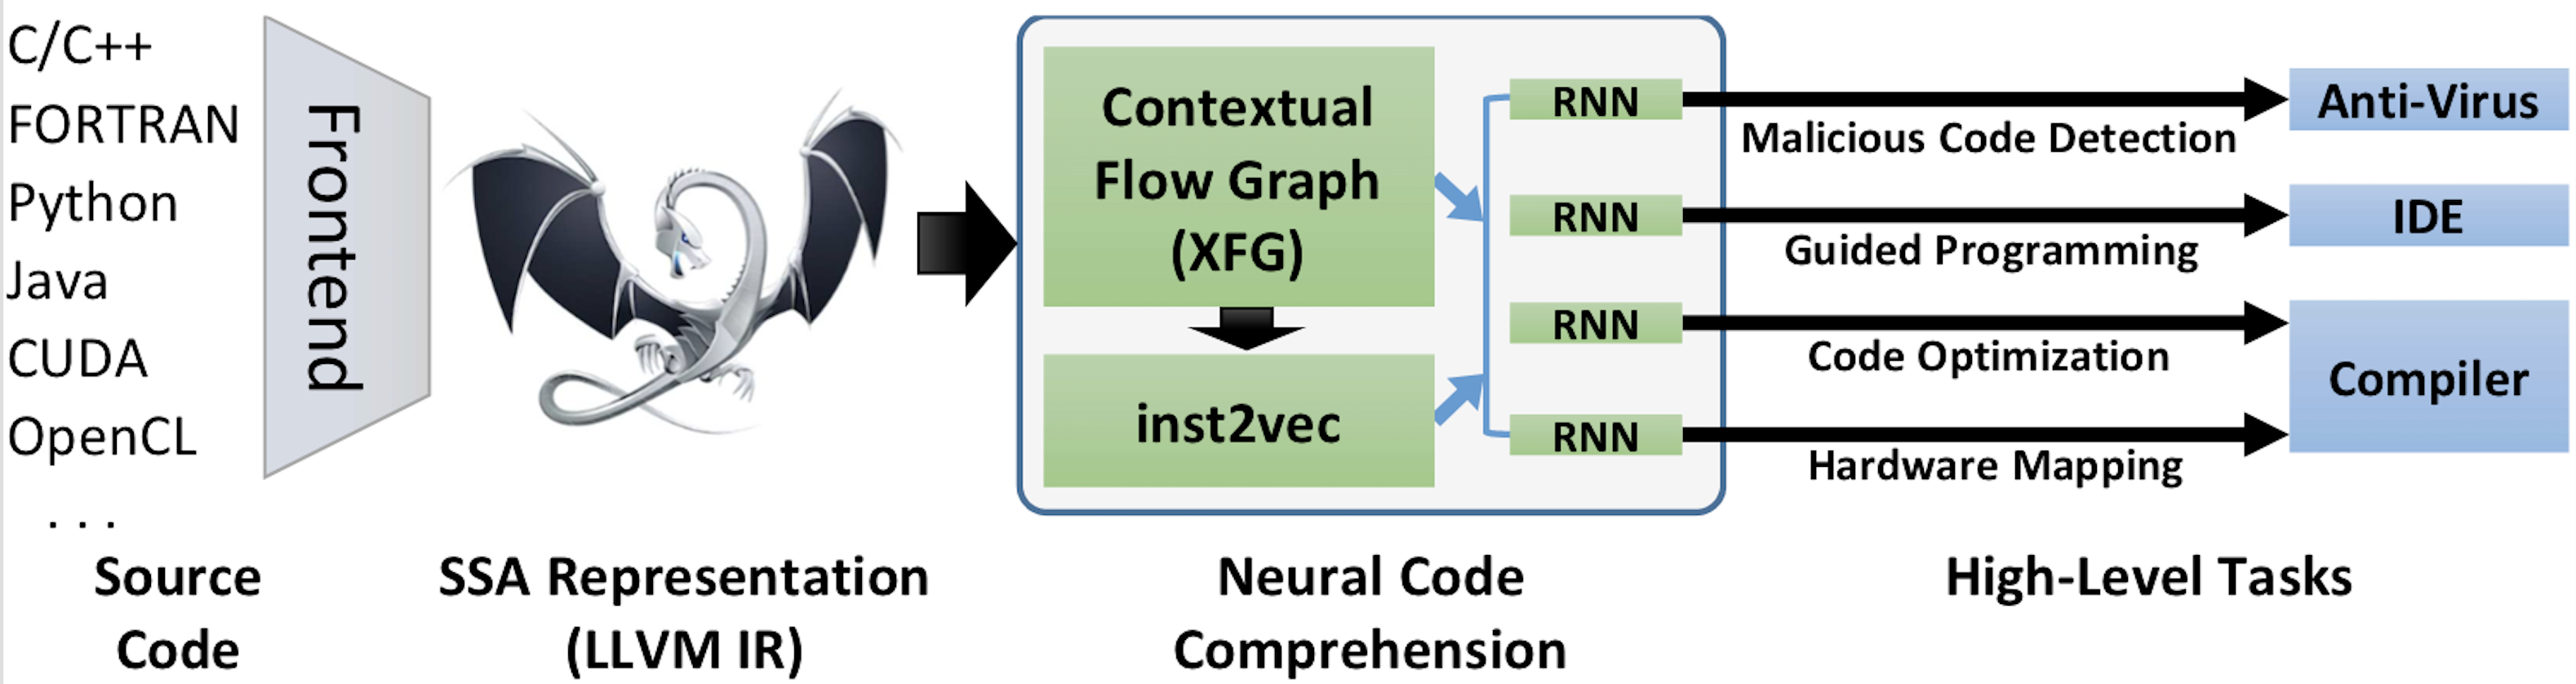
\includegraphics[width=0.9\linewidth]{images/inst2vec.jpg}}
    \caption{Принципиальная схема модели inst2vec}
    \label{ris:inst2vec}
\end{figure}

Данный подход имеет свои плюсы, важнейшими из которых является обобщённость и возможность повторного использования векторных представлений. Также стоит отметить, что этот подход является наиболее простым с вычислительной точки зрения, относительно других подходов, рассмотренных ранее. 
    \section{Сбор набора данных} \label{5-dataset}

Поиск по открытым источникам размеченного набора данных, содержащего бинарный код функций, не дал результатов, поэтому было принято решение подготовить набор данных самостоятельно, используя открытый исходный код проектов на платформе Github. Требовалось выбрать компилируемый язык, на котором в дальнейшем предполагалось собирать проекты. При этом для автоматизации процесса cбора данных необходимо, чтобы процесс сборки проектов был унифицированным. Исходя из описанных требований, был выбран язык Rust, в котором де-факто стандартным инструментом для сборки проектов является Cargo. Чтобы определить набор классов, которым могут принадлежать функции, было решено применить алгоритм кластеризации и посмотреть типичных представителей для каждого кластера. После этого появляется возможность автоматически построить соответствие между скомпилированными функциями и полученными классами, т.е автоматически разметить набор данных. Для построения алгоритма кластеризации использовались сигнатуры функций, методов и комментарии к ним из проектов на языках C/C++/Rust. Код программной реализации находится в открытом доступе\footnote{\url{https://github.com/vladimirtelepov/course-work5}}.

\subsection{Сбор исходных кодов проектов с Github}
Github предоставляет для взаимодействия REST API. Для удобства была использована библиотека PyGithub. Искались репозитории с кодом на языках C/C++/Rust, выдача сортировалась по количеству оценок, брались репозитории с наибольшим количеством оценок. Для кластеризации сохранялись только файлы с расширениями .c, .cpp, .cc, .h, .rs. В итоге был собран код более чем из 16000 репозиториев.

\subsection{Подготовка данных для кластеризации}
Для того чтобы найти сигнатуры функций и комментарии к ним в полученных на предыдущем шаге файлах, использовались библиотеки clang и syn. Для уменьшения времени работы код был распараллелен с помощью библиотек multiprocessing, threading. В результате было собрано более 3.5 миллионов уникальных сигнатур и комментариев.

\subsection{Кластеризация}
Сначала имена функций, семантически состоящие из нескольких частей, разбивались на несколько слов перебором по различным стилям написания (camelCase, underscores, PascalCase). Все слова приводились к нижнему регистру, и удалялись все символы-цифры. Тем не менее по завершении описанных операций оставались слова, семантически состоящие из нескольких частей. Поэтому была произведена сегментация всех полученных ранее слов с помощью алгоритма из книги Beatiful Data\cite{SegaranHammerbacher2009}. Предлагается следующая модель:

Последовательность слов $w_1..w_n$ рассматривается как мешок слов, т.е слова в последовательности считаются независимыми, поэтому $P(w_1...w_n) = P(w_1) * P(w_2) * ... * P(w_n)$. Разбиение слова $w$ на слова $w_1..w_n$ производится с помощью максимизации вероятности наблюдения последовательности слов $w_1..w_s, s <= m,$ где $m$ -- длина слова $w, w = \overline{w_1..w_s}$. Оценка вероятностей встречаемости слов обычно берется из готовых словарей, однако, из-за специфики именования функций, вероятности были оценены подсчетом частоты встречаемости слов в собранном наборе данных. Для того чтобы различать слова, в написании которых есть ошибки, от слов, не встретившихся в корпусе, и присваивать им разные вероятности, применяется аналог сглаживания вероятности Гуда-Тьюринга. Если слово не встретилось в корпусе текста, то будем давать оценку вероятности на основе вероятности встретить слово такой же длины:
Пусть $l$ -- длина слова $w$, не встретившегося в словаре, $P_{ones}(l)$ -- вероятность случайно выбрать слово длины $l$ среди слов, встретившихся в наборе данных один раз, $c_{prior}$ -- константа, позволяющая сделать незнакомые слова менее вероятными, $l_{max}$ -- максимальная длина слова, что $P_{ones}(l_{max}) > 0$. Тогда

$P_{unseen}(w) = \begin{cases}
c_{prior} * P_{ones}(l) & \quad P_{ones}(l) > 0 , \\
c_{prior} * \frac{1}{26}^l & \quad P_{ones}(l) = 0, l < l_{max}, \\
c_{prior} * P_{ones}(l_{max}) * \frac{1}{26}^{(l-l_{max})} & \quad P_{ones}(l) = 0, l >= l_{max}
\end{cases}$

Далее производилась лемматизация для приведения слов к нормальной форме и уменьшения размера словаря. Использовалась библиотека spacy и модель для английского текста. После этого удалялись слишком короткие, длинные, редкие и стоп-слова. Был получен словарь встречаемости, состоящий примерно из 50000 слов. Далее типы аргументов и возвращаемого значения были унифицированы. Затем к полученным векторам токенов применялась модель TF-IDF с логарифмическим преобразованием для TF компоненты. Использовалась библиотека sklearn. После этого применялся алгоритм кластеризации k-means из той же библиотеки, количество кластеров было задано 500. После этого брались "типичные представители" для каждого кластера как ближайшие к центроидам векторы. Алгоритм k-means -- фактически единственный метод, который отработал без превышения лимита по времени/используемым ресурсам на собранном наборе данных.

\subsection{Оценка качества кластеризации}
Для оценки качества кластеризации были просмотрены "значимые" слова в каждом кластере, то есть те, у которых наблюдался наибольший вес при усреднении векторных представлений по всем экземплярам кластера. Неоднократно имела место ситуация, когда 3 самых значимых слова в одном кластере частично совпадают с 3 самыми значимыми словами в другом кластере. Среди полученных кластеров имелись также очень маленькие кластеры и несколько очень больших, которые тяжело интерпретировать. Таким образом, приемлемое качество кластеризации не было достигнуто.

\subsection{Применение других методов обучения без учителя для группировки функций}
Были опробованы методы тематической классификации LSA, PLSA, LDA. Кроме того, были протестированы различные преобразования матрицы tf-idf перед подачей векторов алгоритму k-means: было произведено сокращение размерности пространства с помощью метода главных компонент, токенизированные представления сигнатур подавались предобученной модели BERT, брались значения векторов с последних 4 слоев и усреднялись, затем полученные последовательности усреднялись с помощью взвешивания по tf-idf соответствующей сигнатуры. 

Полученные кластеры также было сложно интерпретировать, поэтому было решено отказаться от методов обучения без учителя и выделить классы вручную.

\subsection{Выделение классов}
Для выделения классов было принято решение оставить только названия функций.
Выделение классов происходило следующим образом:
\begin{enumerate}
    \item просматривался список самых частых слов, из них первые 20-30 слов либо относились к уже выбранным классам или к стоп-словам, либо образовывали новые классы, либо пропускались;
    \item затем производилась разметка всех неразмеченных функций: для каждого класса считалось число слов, входящих в токенизированное название функции (слово может входить несколько раз), и выбирался класс с наибольшим количеством совпадений. При этом как минимум половина слов из названия функции должна была состоять в этом классе. Если таких классов было несколько, то выбирался случайный класс;
    \item далее процесс повторялся. 
\end{enumerate}

В итоге было отобрано 46 классов функций (подробнее про классы см. Приложение). Таким образом удалось разметить 1.5 миллиона функций.

\subsection{Выбор функций и разметка}
После сборки проектов, они компилировались с помощью cargo. Из исходного файла проекта выбирались имена функций. Каждый бинарный файл (ELF-файл, разделяемая или статическая библиотека, библиотека .rlib) подавался на вход программе mcsema-disass. Полученный граф потока управления подавался программе mcsema-lift. В конце биткод переводился в llvm-ir с помощью llvm-dis. В полученном файле искался код функций из исходных файлов с помощью регулярного выражения, содержащего выбранные имена, и сопоставления префикса названия функции и имени бинарного файла. По имени функции, используя описанный выше алгоритм, определялся класс, которому принадлежала функция. Для уменьшения времени работы код был распараллелен с помощью библиотек multiprocessing, threading.


    \section{Описание предлагаемого подхода}
В этом разделе описывается предлагаемый подход к классификации функций.

\subsection{Алгоритм классификации функций в бинарном коде}
Программный комплекс, решающий задачу определения поведения функций, состоит из фреймворков McSema и NCC.

Предлагаемый алгоритм получения меток для каждой функции в бинарном исполняемом файле выглядит следующим образом: 
\begin{enumerate}
    \item На первом этапе исполняемый бинарный файл подается в программу mcsema-disas из фреймворка McSema, из него извлекается граф потока управления;
    \item Полученный на предыдущем шаге файл подается в программу mcsema-lift из фреймворка McSema, который переводит файл в llvm биткод;
    \item Файл с llvm биткодом переводится программой llvm-dis из фреймворка LLVM в представление llvm ir;
    \item Полученный файл подается на вход программы classifyapp. Программа выполняет следующие действия: 
    \begin{enumerate}
        \item Файл с llvm ir разбивается на функции, каждая функция сохраняется в отдельном файле;
        \item Все инструкции в файлах заменяются на их векторные представления (брались предобученные векторы из фреймворка NCC);
        \item Файлы поступают на вход рекуррентной нейронной сети, которая возвращает распределение вероятностей принадлежности функции классам;
        \item Из полученного распределения сохраняются в отдельный файл в json формате 3 меток классов с максимальными вероятностями.
    \end{enumerate}
    \item На последнем шаге с помощью плагина полученный json файл загружается в Ida Pro и для каждой функции создаётся комментарий с 3 полученными метками классов.
\end{enumerate}

Данный алгоритм изображён на рисунке \ref{ris:sugested_approach}.
\begin{figure}[h]
    \center{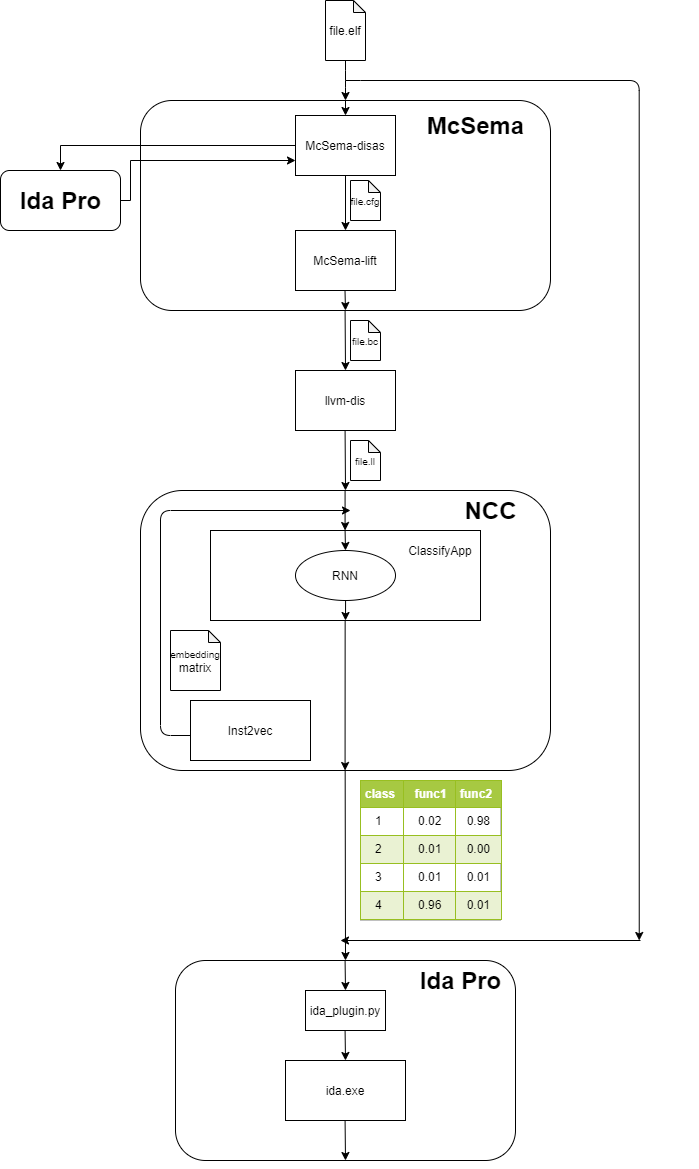
\includegraphics[width=0.70\linewidth,height=0.72\textheight]{images/scheme_vert.png}}
    \caption{Предлагаемый алгоритм классификации функций в бинарном файле}
    \label{ris:sugested_approach}
\end{figure}

\subsection{Обучение рекуррентной нейронной сети}
Рекуррентная нейронная сеть состояла из двух SRU\cite{lei2018simple} блоков, слоя нормализации LayerNorm\cite{LayerNorm} перед каждым SRU блоком, слоя Dropout между SRU блоками и полносвязного слоя. В модели было обучаемых параметров.

В качестве функции ошибки использовалась функция cross-entropy loss и метод оптимизации Adam.

Все последовательности дополнялись до 830 токенов или обрезались, если их длина была больше.

Перебор гиперпараметров производился с помощью алгоритма ASHA\cite{li2018massively}.

Код программной реализации находится в открытом доступе\footnote{\url{https://github.com/vladimirtelepov/ncc}}

\subsection{Результаты обучения рекуррентной нейронной сети}
Была получена доля верно угаданных меток $\%$ на тренировочной выборке, $\%$ на валидационной выборке и $\%$ на тестовой выборке, графики зависимостей от количества эпох можно увидеть на рисунках \ref{ris:loss} и \ref{ris:acc}. На обоих рисунках синяя линия соответствует тренировочной выборке, желтая - валидационной.

\subsection{Ограничения подхода}
Из предыдущей секции можно сделать вывод о том, что предложенный подход применим для анализа больших бинарных программ и сложных алгоритмов. Однако у данного подхода есть следующие ограничения:
\begin{enumerate}
    \item Mcsema не всегда может перевести в llvm ir бинарный файл, и результат ее работы сильно зависит от дизассемблера. Также нужно учесть, что результат работы дизассемблера для обфусцированных бинарных файлов может быть неудовлетворительным, и, следовательно, данный подход не может быть применён;
    \item Структура полученного .ll файла очень сильно зависит от работы mcsema, поэтому при значительных изменениях ее ядра необходимо заново переобучать рекуррентную нейронную сеть.
\end{enumerate}
\newpage
    \section*{Заключение}
Основные результаты данной работы заключаются в следующем:
\begin{enumerate}
    \item Была исследованы подходы по распознаванию семантики кода, использующие в своей основе нейронные сети;
    \item Был собран набор данных из проектов с платформы Github;
    \item Был предложен и реализован алгоритм кластеризации сигнатур функций из этих проектов;
    \item Был декомпилирован и размечен в соответствии с работой алгоритма кластеризации собранный набор данных;
    \item Был проверен метод классификации функций в исполняемых бинарных файлах.
\end{enumerate}
}


% Информация о годе выполнения работы
\def\Year{%
    2022%
    % \the\year%     % Текущий год
}

% Укажите тип работы
% Например:
%     Выпускная квалификационная работа,
%     Магистерская диссертация,
%     Курсовая работа, реферат и т.п.
\def\WorkType{%
    % Выпускная квалификационная работа%
    Магистерская диссертация
    % Курсовая работа%
    % Реферат%
    % Дипломная работа%
}

% Название работы
%%%%%%%%%%% ВНИМАНИЕ! %%%%%%%%%%%%%%%%
% В МГУ ОНО ДОЛЖНО В ТОЧНОСТИ
% СООТВЕТСТВОВАТЬ ВЫПИСКЕ ИЗ ПРИКАЗА
% УТОЧНИТЕ НАЗВАНИЕ В УЧЕБНОЙ ЧАСТИ
\def\Title{%
    Исследование способов классификации функций в бинарных исполняемых файлах%
}


% Имя автора работы
\def\Author{%
    Телепов Владимир Юрьевич%
}

% Информация о научном руководителе
%% Фамилия Имя Отчество%
\def\SciAdvisor{%
    Гамаюнов Денис Юрьевич%
    % Воронов Михаил Серегеевич%
}
%% В формате: И.~О.~Фамилия%
\def\SciAdvisorShort{%
    Д.~Ю.~Гамаюнов%
    % М.~С.~Воронов%
}
%% должность научного руководителя
\def\Position{%
    % профессор%
    % доцент%
    % старший преподаватель%
    % преподаватель%
    % ассистент%
    % ведущий научный сотрудник%
    старший научный сотрудник%
    % научный сотрудник%
    % младший научный сотрудник%
    % сотрудник ЛБИС%
}
%% учёная степень научного руководителя
\def\AcademicDegree{%
    % д.ф.-м.н.%
    % д.т.н.%
    к.ф.-м.н.%
    % к.т.н.%
    % без степени%
}

% Информация об организации, в которой выполнена работа
%% Город
\def\Place{%
    Москва%
}
%% Университет
\def\Univer{%
    Московский государственный университет имени М.~В.~Ломоносова%
}
%% Факультет
\def\Faculty{%
    Факультет вычислительной математики и кибернетики%
}
%% Кафедра    
\def\Department{%
    Кафедра информационной безопасности%
}     

%%%% Переключите статус документа для отладки
%%%% В режиме draft документ собирается очень быстро
%%%% и выводится полезная информация о том
%%%% какие строки вылезают за границы документа, что удобно для борьбы с ними
\def\Status{%
    % draft%
    final%
}

%%%% Включает и выключает подпись <<С текстом работы ознакомлен>>
\def\EnableSign{%
    % true%
}
